\documentclass[twoside]{article}

% Packages required by doxygen
\usepackage{calc}
\usepackage{doxygen}
\usepackage{graphicx}
\usepackage[utf8]{inputenc}
\usepackage{makeidx}
\usepackage{multicol}
\usepackage{multirow}
\usepackage{textcomp}
\usepackage[table]{xcolor}

% Font selection
\usepackage[T1]{fontenc}
\usepackage{mathptmx}
\usepackage[scaled=.90]{helvet}
\usepackage{courier}
\usepackage{amssymb}
\usepackage{sectsty}
\renewcommand{\familydefault}{\sfdefault}
\allsectionsfont{%
  \fontseries{bc}\selectfont%
  \color{darkgray}%
}
\renewcommand{\DoxyLabelFont}{%
  \fontseries{bc}\selectfont%
  \color{darkgray}%
}

% Page & text layout
\usepackage{geometry}
\geometry{%
  a4paper,%
  top=2.5cm,%
  bottom=2.5cm,%
  left=2.5cm,%
  right=2.5cm%
}
\tolerance=750
\hfuzz=15pt
\hbadness=750
\setlength{\emergencystretch}{15pt}
\setlength{\parindent}{0cm}
\setlength{\parskip}{0.2cm}
\makeatletter
\renewcommand{\paragraph}{%
  \@startsection{paragraph}{4}{0ex}{-1.0ex}{1.0ex}{%
    \normalfont\normalsize\bfseries\SS@parafont%
  }%
}
\renewcommand{\subparagraph}{%
  \@startsection{subparagraph}{5}{0ex}{-1.0ex}{1.0ex}{%
    \normalfont\normalsize\bfseries\SS@subparafont%
  }%
}
\makeatother

% Headers & footers
\usepackage{fancyhdr}
\pagestyle{fancyplain}
\fancyhead[LE]{\fancyplain{}{\bfseries\thepage}}
\fancyhead[CE]{\fancyplain{}{}}
\fancyhead[RE]{\fancyplain{}{\bfseries\leftmark}}
\fancyhead[LO]{\fancyplain{}{\bfseries\rightmark}}
\fancyhead[CO]{\fancyplain{}{}}
\fancyhead[RO]{\fancyplain{}{\bfseries\thepage}}
\fancyfoot[LE]{\fancyplain{}{}}
\fancyfoot[CE]{\fancyplain{}{}}
\fancyfoot[RE]{\fancyplain{}{\bfseries\scriptsize Generated on Thu May 22 2014 20\-:52\-:51 for Soundlie\-: User Interface Source Code by Doxygen }}
\fancyfoot[LO]{\fancyplain{}{\bfseries\scriptsize Generated on Thu May 22 2014 20\-:52\-:51 for Soundlie\-: User Interface Source Code by Doxygen }}
\fancyfoot[CO]{\fancyplain{}{}}
\fancyfoot[RO]{\fancyplain{}{}}
\renewcommand{\footrulewidth}{0.4pt}
\renewcommand{\sectionmark}[1]{%
  \markright{\thesection\ #1}%
}

% Indices & bibliography
\usepackage{natbib}
\usepackage[titles]{tocloft}
\setcounter{tocdepth}{3}
\setcounter{secnumdepth}{5}
\makeindex

% Hyperlinks (required, but should be loaded last)
\usepackage{ifpdf}
\ifpdf
  \usepackage[pdftex,pagebackref=true]{hyperref}
\else
  \usepackage[ps2pdf,pagebackref=true]{hyperref}
\fi
\hypersetup{%
  colorlinks=true,%
  linkcolor=blue,%
  citecolor=blue,%
  unicode%
}

% Custom commands
\newcommand{\clearemptydoublepage}{%
  \newpage{\pagestyle{empty}\cleardoublepage}%
}


%===== C O N T E N T S =====

\begin{document}

% Titlepage & ToC
\hypersetup{pageanchor=false}
\pagenumbering{roman}
\begin{titlepage}
\vspace*{7cm}
\begin{center}%
{\Large Soundlie\-: User Interface Source Code \\[1ex]\large 1.\-0 }\\
\vspace*{1cm}
{\large Generated by Doxygen 1.8.6}\\
\vspace*{0.5cm}
{\small Thu May 22 2014 20:52:51}\\
\end{center}
\end{titlepage}
\tableofcontents
\pagenumbering{arabic}
\hypersetup{pageanchor=true}

%--- Begin generated contents ---
\section{Namespace Index}
\subsection{Namespace List}
Here is a list of all namespaces with brief descriptions\-:\begin{DoxyCompactList}
\item\contentsline{section}{\hyperlink{namespaceuart__gui}{uart\-\_\-gui} }{\pageref{d9/d5d/namespaceuart__gui}}{}
\item\contentsline{section}{\hyperlink{namespaceuart__gui_1_1_properties}{uart\-\_\-gui.\-Properties} }{\pageref{d2/d60/namespaceuart__gui_1_1_properties}}{}
\end{DoxyCompactList}

\section{Hierarchical Index}
\subsection{Class Hierarchy}
This inheritance list is sorted roughly, but not completely, alphabetically\-:\begin{DoxyCompactList}
\item Form\begin{DoxyCompactList}
\item \contentsline{section}{uart\-\_\-gui.\-Soundlie\-\_\-\-G\-U\-I}{\pageref{d0/dc1/classuart__gui_1_1_soundlie___g_u_i}}{}
\end{DoxyCompactList}
\item \contentsline{section}{uart\-\_\-gui.\-Program}{\pageref{d2/dc4/classuart__gui_1_1_program}}{}
\end{DoxyCompactList}

\section{Data Structure Index}
\subsection{Data Structures}
Here are the data structures with brief descriptions\-:\begin{DoxyCompactList}
\item\contentsline{section}{\hyperlink{classuart__gui_1_1_program}{uart\-\_\-gui.\-Program} }{\pageref{d2/dc4/classuart__gui_1_1_program}}{}
\item\contentsline{section}{\hyperlink{classuart__gui_1_1_soundlie___g_u_i}{uart\-\_\-gui.\-Soundlie\-\_\-\-G\-U\-I} \\*Form1 G\-U\-I class }{\pageref{d0/dc1/classuart__gui_1_1_soundlie___g_u_i}}{}
\end{DoxyCompactList}

\section{File Index}
\subsection{File List}
Here is a list of all files with brief descriptions\-:\begin{DoxyCompactList}
\item\contentsline{section}{\hyperlink{_assembly_info_8cs}{Assembly\-Info.\-cs} }{\pageref{d7/d2f/_assembly_info_8cs}}{}
\item\contentsline{section}{\hyperlink{_program_8cs}{Program.\-cs} }{\pageref{dd/d5c/_program_8cs}}{}
\item\contentsline{section}{\hyperlink{_resources_8_designer_8cs}{Resources.\-Designer.\-cs} }{\pageref{d6/d0e/_resources_8_designer_8cs}}{}
\item\contentsline{section}{\hyperlink{_settings_8_designer_8cs}{Settings.\-Designer.\-cs} }{\pageref{d1/d1c/_settings_8_designer_8cs}}{}
\item\contentsline{section}{\hyperlink{_soundlie___g_u_i_8cs}{Soundlie\-\_\-\-G\-U\-I.\-cs} }{\pageref{d6/d80/_soundlie___g_u_i_8cs}}{}
\item\contentsline{section}{\hyperlink{_soundlie___g_u_i_8_designer_8cs}{Soundlie\-\_\-\-G\-U\-I.\-Designer.\-cs} }{\pageref{de/d0d/_soundlie___g_u_i_8_designer_8cs}}{}
\item\contentsline{section}{\hyperlink{_temporary_generated_file__036_c0_b5_b-1481-4323-8_d20-8_f5_a_d_c_b23_d92_8cs}{Temporary\-Generated\-File\-\_\-036\-C0\-B5\-B-\/1481-\/4323-\/8\-D20-\/8\-F5\-A\-D\-C\-B23\-D92.\-cs} }{\pageref{df/d63/_temporary_generated_file__036_c0_b5_b-1481-4323-8_d20-8_f5_a_d_c_b23_d92_8cs}}{}
\item\contentsline{section}{\hyperlink{_temporary_generated_file__5937a670-0e60-4077-877b-f7221da3dda1_8cs}{Temporary\-Generated\-File\-\_\-5937a670-\/0e60-\/4077-\/877b-\/f7221da3dda1.\-cs} }{\pageref{db/d59/_temporary_generated_file__5937a670-0e60-4077-877b-f7221da3dda1_8cs}}{}
\item\contentsline{section}{\hyperlink{_temporary_generated_file___e7_a71_f73-0_f8_d-4_b9_b-_b56_e-8_e70_b10_b_c5_d3_8cs}{Temporary\-Generated\-File\-\_\-\-E7\-A71\-F73-\/0\-F8\-D-\/4\-B9\-B-\/\-B56\-E-\/8\-E70\-B10\-B\-C5\-D3.\-cs} }{\pageref{de/d44/_temporary_generated_file___e7_a71_f73-0_f8_d-4_b9_b-_b56_e-8_e70_b10_b_c5_d3_8cs}}{}
\end{DoxyCompactList}

\section{Namespace Documentation}
\hypertarget{namespaceuart__gui}{\subsection{Package uart\-\_\-gui}
\label{namespaceuart__gui}\index{uart\-\_\-gui@{uart\-\_\-gui}}
}
\subsubsection*{Namespaces}
\begin{DoxyCompactItemize}
\item 
package \hyperlink{namespaceuart__gui_1_1_properties}{Properties}
\end{DoxyCompactItemize}
\subsubsection*{Data Structures}
\begin{DoxyCompactItemize}
\item 
class \hyperlink{classuart__gui_1_1_program}{Program}
\item 
class \hyperlink{classuart__gui_1_1_soundlie___g_u_i}{Soundlie\-\_\-\-G\-U\-I}
\begin{DoxyCompactList}\small\item\em Form1 G\-U\-I class. \end{DoxyCompactList}\end{DoxyCompactItemize}

\hypertarget{namespaceuart__gui_1_1_properties}{\subsection{Package uart\-\_\-gui.\-Properties}
\label{namespaceuart__gui_1_1_properties}\index{uart\-\_\-gui.\-Properties@{uart\-\_\-gui.\-Properties}}
}
\subsubsection*{Data Structures}
\begin{DoxyCompactItemize}
\item 
class {\bfseries Resources}
\begin{DoxyCompactList}\small\item\em A strongly-\/typed resource class, for looking up localized strings, etc. \end{DoxyCompactList}\item 
class {\bfseries Settings}
\end{DoxyCompactItemize}

\section{Data Structure Documentation}
\hypertarget{classuart__gui_1_1_program}{\subsection{uart\-\_\-gui.\-Program Class Reference}
\label{classuart__gui_1_1_program}\index{uart\-\_\-gui.\-Program@{uart\-\_\-gui.\-Program}}
}


Collaboration diagram for uart\-\_\-gui.\-Program\-:\nopagebreak
\begin{figure}[H]
\begin{center}
\leavevmode
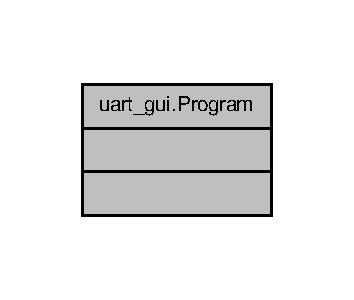
\includegraphics[width=170pt]{d3/dd1/classuart__gui_1_1_program__coll__graph}
\end{center}
\end{figure}


The documentation for this class was generated from the following file\-:\begin{DoxyCompactItemize}
\item 
\hyperlink{_program_8cs}{Program.\-cs}\end{DoxyCompactItemize}

\hypertarget{classuart__gui_1_1_soundlie___g_u_i}{\subsection{uart\-\_\-gui.\-Soundlie\-\_\-\-G\-U\-I Class Reference}
\label{classuart__gui_1_1_soundlie___g_u_i}\index{uart\-\_\-gui.\-Soundlie\-\_\-\-G\-U\-I@{uart\-\_\-gui.\-Soundlie\-\_\-\-G\-U\-I}}
}


Form1 G\-U\-I class.  




Inheritance diagram for uart\-\_\-gui.\-Soundlie\-\_\-\-G\-U\-I\-:\nopagebreak
\begin{figure}[H]
\begin{center}
\leavevmode
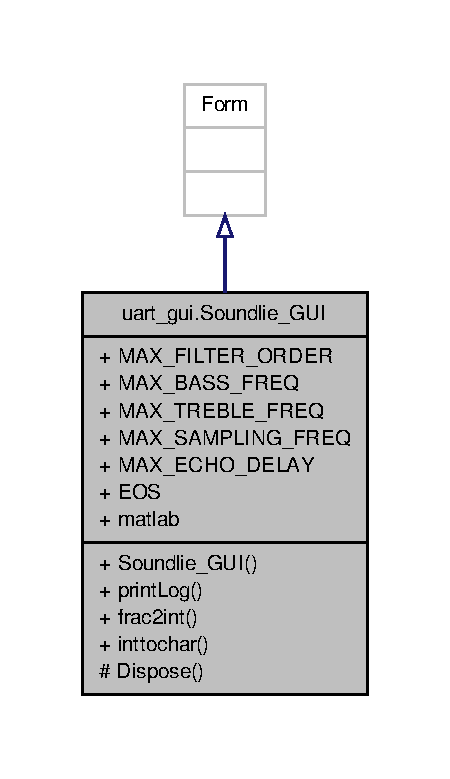
\includegraphics[width=216pt]{df/d32/classuart__gui_1_1_soundlie___g_u_i__inherit__graph}
\end{center}
\end{figure}


Collaboration diagram for uart\-\_\-gui.\-Soundlie\-\_\-\-G\-U\-I\-:\nopagebreak
\begin{figure}[H]
\begin{center}
\leavevmode
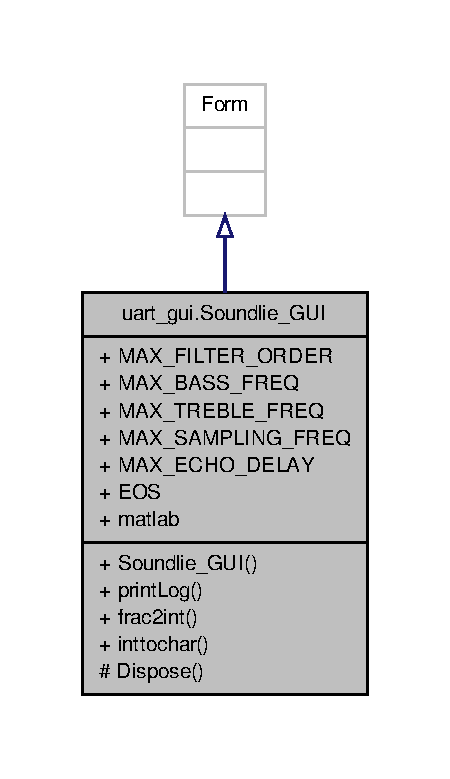
\includegraphics[width=216pt]{d2/dd1/classuart__gui_1_1_soundlie___g_u_i__coll__graph}
\end{center}
\end{figure}
\subsubsection*{Public Member Functions}
\begin{DoxyCompactItemize}
\item 
\hyperlink{classuart__gui_1_1_soundlie___g_u_i_a6fa0299c3a671064f9409fd7cf591a19}{Soundlie\-\_\-\-G\-U\-I} ()
\item 
void \hyperlink{classuart__gui_1_1_soundlie___g_u_i_abc7db78994d56752133d9cc62938da81}{print\-Log} (string s, bool time=true)
\end{DoxyCompactItemize}
\subsubsection*{Static Public Member Functions}
\begin{DoxyCompactItemize}
\item 
static Int16 \hyperlink{classuart__gui_1_1_soundlie___g_u_i_aa200a65d9bc20ba4625be9c02fb7c4b3}{frac2int} (float f)
\item 
static char \hyperlink{classuart__gui_1_1_soundlie___g_u_i_a1ade5c03bb1f55b814fdc396e4982f72}{inttochar} (int num)
\end{DoxyCompactItemize}
\subsubsection*{Data Fields}
\begin{DoxyCompactItemize}
\item 
const Int16 \hyperlink{classuart__gui_1_1_soundlie___g_u_i_a30cbbba38c4151c2e85354e467fa956d}{M\-A\-X\-\_\-\-F\-I\-L\-T\-E\-R\-\_\-\-O\-R\-D\-E\-R} = 5
\begin{DoxyCompactList}\small\item\em maximum number of filter taps \end{DoxyCompactList}\item 
const Int16 \hyperlink{classuart__gui_1_1_soundlie___g_u_i_ac90d2c11617fac149686285a050a30b6}{M\-A\-X\-\_\-\-B\-A\-S\-S\-\_\-\-F\-R\-E\-Q} = 10000
\begin{DoxyCompactList}\small\item\em highest B\-A\-S\-S (L\-P) filter frequency \end{DoxyCompactList}\item 
const Int16 \hyperlink{classuart__gui_1_1_soundlie___g_u_i_aca72413113098188452107bf8f041b55}{M\-A\-X\-\_\-\-T\-R\-E\-B\-L\-E\-\_\-\-F\-R\-E\-Q} = 30000
\begin{DoxyCompactList}\small\item\em highest T\-R\-E\-B\-L\-E (H\-P) filter frequency \end{DoxyCompactList}\item 
const Int32 \hyperlink{classuart__gui_1_1_soundlie___g_u_i_a68f81db8e078a384454f91418d450e0f}{M\-A\-X\-\_\-\-S\-A\-M\-P\-L\-I\-N\-G\-\_\-\-F\-R\-E\-Q} = 50000
\begin{DoxyCompactList}\small\item\em highest sampling frequency \end{DoxyCompactList}\item 
const Int32 \hyperlink{classuart__gui_1_1_soundlie___g_u_i_a5ec140dda2bb623d2841d307ff8ee9bf}{M\-A\-X\-\_\-\-E\-C\-H\-O\-\_\-\-D\-E\-L\-A\-Y} = 48000
\begin{DoxyCompactList}\small\item\em highest E\-C\-H\-O delay \end{DoxyCompactList}\item 
const Char \hyperlink{classuart__gui_1_1_soundlie___g_u_i_a6d2c148b379977b23fc0b1c56ee7e1c3}{E\-O\-S} = 'x'
\begin{DoxyCompactList}\small\item\em end-\/of-\/sequency used for the U\-A\-R\-T message \end{DoxyCompactList}\item 
M\-L\-App.\-M\-L\-App \hyperlink{classuart__gui_1_1_soundlie___g_u_i_a3e31d22444514a602e98334ffd0db8a0}{matlab}
\begin{DoxyCompactList}\small\item\em Mat\-L\-A\-B C\-O\-M object. \end{DoxyCompactList}\end{DoxyCompactItemize}
\subsubsection*{Protected Member Functions}
\begin{DoxyCompactItemize}
\item 
override void \hyperlink{classuart__gui_1_1_soundlie___g_u_i_ab8716ab8b8d492fb9a25d82dcc799c4d}{Dispose} (bool disposing)
\begin{DoxyCompactList}\small\item\em Clean up any resources being used. \end{DoxyCompactList}\end{DoxyCompactItemize}


\subsubsection{Detailed Description}
Form1 G\-U\-I class. 

Form1 class mapping all the G\-U\-I functionality0. 

\subsubsection{Constructor \& Destructor Documentation}
\hypertarget{classuart__gui_1_1_soundlie___g_u_i_a6fa0299c3a671064f9409fd7cf591a19}{\index{uart\-\_\-gui\-::\-Soundlie\-\_\-\-G\-U\-I@{uart\-\_\-gui\-::\-Soundlie\-\_\-\-G\-U\-I}!Soundlie\-\_\-\-G\-U\-I@{Soundlie\-\_\-\-G\-U\-I}}
\index{Soundlie\-\_\-\-G\-U\-I@{Soundlie\-\_\-\-G\-U\-I}!uart_gui::Soundlie_GUI@{uart\-\_\-gui\-::\-Soundlie\-\_\-\-G\-U\-I}}
\paragraph[{Soundlie\-\_\-\-G\-U\-I}]{\setlength{\rightskip}{0pt plus 5cm}uart\-\_\-gui.\-Soundlie\-\_\-\-G\-U\-I.\-Soundlie\-\_\-\-G\-U\-I (
\begin{DoxyParamCaption}
{}
\end{DoxyParamCaption}
)\hspace{0.3cm}{\ttfamily [inline]}}}\label{classuart__gui_1_1_soundlie___g_u_i_a6fa0299c3a671064f9409fd7cf591a19}


\subsubsection{Member Function Documentation}
\hypertarget{classuart__gui_1_1_soundlie___g_u_i_ab8716ab8b8d492fb9a25d82dcc799c4d}{\index{uart\-\_\-gui\-::\-Soundlie\-\_\-\-G\-U\-I@{uart\-\_\-gui\-::\-Soundlie\-\_\-\-G\-U\-I}!Dispose@{Dispose}}
\index{Dispose@{Dispose}!uart_gui::Soundlie_GUI@{uart\-\_\-gui\-::\-Soundlie\-\_\-\-G\-U\-I}}
\paragraph[{Dispose}]{\setlength{\rightskip}{0pt plus 5cm}override void uart\-\_\-gui.\-Soundlie\-\_\-\-G\-U\-I.\-Dispose (
\begin{DoxyParamCaption}
\item[{bool}]{disposing}
\end{DoxyParamCaption}
)\hspace{0.3cm}{\ttfamily [inline]}, {\ttfamily [protected]}}}\label{classuart__gui_1_1_soundlie___g_u_i_ab8716ab8b8d492fb9a25d82dcc799c4d}


Clean up any resources being used. 


\begin{DoxyParams}{Parameters}
{\em disposing} & true if managed resources should be disposed; otherwise, false.\\
\hline
\end{DoxyParams}
\hypertarget{classuart__gui_1_1_soundlie___g_u_i_aa200a65d9bc20ba4625be9c02fb7c4b3}{\index{uart\-\_\-gui\-::\-Soundlie\-\_\-\-G\-U\-I@{uart\-\_\-gui\-::\-Soundlie\-\_\-\-G\-U\-I}!frac2int@{frac2int}}
\index{frac2int@{frac2int}!uart_gui::Soundlie_GUI@{uart\-\_\-gui\-::\-Soundlie\-\_\-\-G\-U\-I}}
\paragraph[{frac2int}]{\setlength{\rightskip}{0pt plus 5cm}static Int16 uart\-\_\-gui.\-Soundlie\-\_\-\-G\-U\-I.\-frac2int (
\begin{DoxyParamCaption}
\item[{float}]{f}
\end{DoxyParamCaption}
)\hspace{0.3cm}{\ttfamily [inline]}, {\ttfamily [static]}}}\label{classuart__gui_1_1_soundlie___g_u_i_aa200a65d9bc20ba4625be9c02fb7c4b3}
Converts a float value to a Q2.\-14 integer representation. 
\begin{DoxyParams}[1]{Parameters}
\mbox{\tt in}  & {\em f} & Value to be converted \\
\hline
\end{DoxyParams}
\begin{DoxyReturn}{Returns}
an integer representation of the float value 
\end{DoxyReturn}
\hypertarget{classuart__gui_1_1_soundlie___g_u_i_a1ade5c03bb1f55b814fdc396e4982f72}{\index{uart\-\_\-gui\-::\-Soundlie\-\_\-\-G\-U\-I@{uart\-\_\-gui\-::\-Soundlie\-\_\-\-G\-U\-I}!inttochar@{inttochar}}
\index{inttochar@{inttochar}!uart_gui::Soundlie_GUI@{uart\-\_\-gui\-::\-Soundlie\-\_\-\-G\-U\-I}}
\paragraph[{inttochar}]{\setlength{\rightskip}{0pt plus 5cm}static char uart\-\_\-gui.\-Soundlie\-\_\-\-G\-U\-I.\-inttochar (
\begin{DoxyParamCaption}
\item[{int}]{num}
\end{DoxyParamCaption}
)\hspace{0.3cm}{\ttfamily [inline]}, {\ttfamily [static]}}}\label{classuart__gui_1_1_soundlie___g_u_i_a1ade5c03bb1f55b814fdc396e4982f72}
Convert an integer ( $<$ 16) to the hex char 
\begin{DoxyParams}[1]{Parameters}
\mbox{\tt in}  & {\em amplification} & string containing the amplification \\
\hline
\end{DoxyParams}
\begin{DoxyReturn}{Returns}
hexadecimal value as a character 
\end{DoxyReturn}
\hypertarget{classuart__gui_1_1_soundlie___g_u_i_abc7db78994d56752133d9cc62938da81}{\index{uart\-\_\-gui\-::\-Soundlie\-\_\-\-G\-U\-I@{uart\-\_\-gui\-::\-Soundlie\-\_\-\-G\-U\-I}!print\-Log@{print\-Log}}
\index{print\-Log@{print\-Log}!uart_gui::Soundlie_GUI@{uart\-\_\-gui\-::\-Soundlie\-\_\-\-G\-U\-I}}
\paragraph[{print\-Log}]{\setlength{\rightskip}{0pt plus 5cm}void uart\-\_\-gui.\-Soundlie\-\_\-\-G\-U\-I.\-print\-Log (
\begin{DoxyParamCaption}
\item[{string}]{s, }
\item[{bool}]{time = {\ttfamily true}}
\end{DoxyParamCaption}
)\hspace{0.3cm}{\ttfamily [inline]}}}\label{classuart__gui_1_1_soundlie___g_u_i_abc7db78994d56752133d9cc62938da81}
Prints data in the G\-U\-I Log. 
\begin{DoxyParams}[1]{Parameters}
\mbox{\tt in}  & {\em s} & string to be printed \\
\hline
\mbox{\tt in}  & {\em time} & true if the log message should have a time stamp \\
\hline
\end{DoxyParams}


\subsubsection{Field Documentation}
\hypertarget{classuart__gui_1_1_soundlie___g_u_i_a6d2c148b379977b23fc0b1c56ee7e1c3}{\index{uart\-\_\-gui\-::\-Soundlie\-\_\-\-G\-U\-I@{uart\-\_\-gui\-::\-Soundlie\-\_\-\-G\-U\-I}!E\-O\-S@{E\-O\-S}}
\index{E\-O\-S@{E\-O\-S}!uart_gui::Soundlie_GUI@{uart\-\_\-gui\-::\-Soundlie\-\_\-\-G\-U\-I}}
\paragraph[{E\-O\-S}]{\setlength{\rightskip}{0pt plus 5cm}const Char uart\-\_\-gui.\-Soundlie\-\_\-\-G\-U\-I.\-E\-O\-S = 'x'}}\label{classuart__gui_1_1_soundlie___g_u_i_a6d2c148b379977b23fc0b1c56ee7e1c3}


end-\/of-\/sequency used for the U\-A\-R\-T message 

\hypertarget{classuart__gui_1_1_soundlie___g_u_i_a3e31d22444514a602e98334ffd0db8a0}{\index{uart\-\_\-gui\-::\-Soundlie\-\_\-\-G\-U\-I@{uart\-\_\-gui\-::\-Soundlie\-\_\-\-G\-U\-I}!matlab@{matlab}}
\index{matlab@{matlab}!uart_gui::Soundlie_GUI@{uart\-\_\-gui\-::\-Soundlie\-\_\-\-G\-U\-I}}
\paragraph[{matlab}]{\setlength{\rightskip}{0pt plus 5cm}M\-L\-App.\-M\-L\-App uart\-\_\-gui.\-Soundlie\-\_\-\-G\-U\-I.\-matlab}}\label{classuart__gui_1_1_soundlie___g_u_i_a3e31d22444514a602e98334ffd0db8a0}


Mat\-L\-A\-B C\-O\-M object. 

\hypertarget{classuart__gui_1_1_soundlie___g_u_i_ac90d2c11617fac149686285a050a30b6}{\index{uart\-\_\-gui\-::\-Soundlie\-\_\-\-G\-U\-I@{uart\-\_\-gui\-::\-Soundlie\-\_\-\-G\-U\-I}!M\-A\-X\-\_\-\-B\-A\-S\-S\-\_\-\-F\-R\-E\-Q@{M\-A\-X\-\_\-\-B\-A\-S\-S\-\_\-\-F\-R\-E\-Q}}
\index{M\-A\-X\-\_\-\-B\-A\-S\-S\-\_\-\-F\-R\-E\-Q@{M\-A\-X\-\_\-\-B\-A\-S\-S\-\_\-\-F\-R\-E\-Q}!uart_gui::Soundlie_GUI@{uart\-\_\-gui\-::\-Soundlie\-\_\-\-G\-U\-I}}
\paragraph[{M\-A\-X\-\_\-\-B\-A\-S\-S\-\_\-\-F\-R\-E\-Q}]{\setlength{\rightskip}{0pt plus 5cm}const Int16 uart\-\_\-gui.\-Soundlie\-\_\-\-G\-U\-I.\-M\-A\-X\-\_\-\-B\-A\-S\-S\-\_\-\-F\-R\-E\-Q = 10000}}\label{classuart__gui_1_1_soundlie___g_u_i_ac90d2c11617fac149686285a050a30b6}


highest B\-A\-S\-S (L\-P) filter frequency 

\hypertarget{classuart__gui_1_1_soundlie___g_u_i_a5ec140dda2bb623d2841d307ff8ee9bf}{\index{uart\-\_\-gui\-::\-Soundlie\-\_\-\-G\-U\-I@{uart\-\_\-gui\-::\-Soundlie\-\_\-\-G\-U\-I}!M\-A\-X\-\_\-\-E\-C\-H\-O\-\_\-\-D\-E\-L\-A\-Y@{M\-A\-X\-\_\-\-E\-C\-H\-O\-\_\-\-D\-E\-L\-A\-Y}}
\index{M\-A\-X\-\_\-\-E\-C\-H\-O\-\_\-\-D\-E\-L\-A\-Y@{M\-A\-X\-\_\-\-E\-C\-H\-O\-\_\-\-D\-E\-L\-A\-Y}!uart_gui::Soundlie_GUI@{uart\-\_\-gui\-::\-Soundlie\-\_\-\-G\-U\-I}}
\paragraph[{M\-A\-X\-\_\-\-E\-C\-H\-O\-\_\-\-D\-E\-L\-A\-Y}]{\setlength{\rightskip}{0pt plus 5cm}const Int32 uart\-\_\-gui.\-Soundlie\-\_\-\-G\-U\-I.\-M\-A\-X\-\_\-\-E\-C\-H\-O\-\_\-\-D\-E\-L\-A\-Y = 48000}}\label{classuart__gui_1_1_soundlie___g_u_i_a5ec140dda2bb623d2841d307ff8ee9bf}


highest E\-C\-H\-O delay 

\hypertarget{classuart__gui_1_1_soundlie___g_u_i_a30cbbba38c4151c2e85354e467fa956d}{\index{uart\-\_\-gui\-::\-Soundlie\-\_\-\-G\-U\-I@{uart\-\_\-gui\-::\-Soundlie\-\_\-\-G\-U\-I}!M\-A\-X\-\_\-\-F\-I\-L\-T\-E\-R\-\_\-\-O\-R\-D\-E\-R@{M\-A\-X\-\_\-\-F\-I\-L\-T\-E\-R\-\_\-\-O\-R\-D\-E\-R}}
\index{M\-A\-X\-\_\-\-F\-I\-L\-T\-E\-R\-\_\-\-O\-R\-D\-E\-R@{M\-A\-X\-\_\-\-F\-I\-L\-T\-E\-R\-\_\-\-O\-R\-D\-E\-R}!uart_gui::Soundlie_GUI@{uart\-\_\-gui\-::\-Soundlie\-\_\-\-G\-U\-I}}
\paragraph[{M\-A\-X\-\_\-\-F\-I\-L\-T\-E\-R\-\_\-\-O\-R\-D\-E\-R}]{\setlength{\rightskip}{0pt plus 5cm}const Int16 uart\-\_\-gui.\-Soundlie\-\_\-\-G\-U\-I.\-M\-A\-X\-\_\-\-F\-I\-L\-T\-E\-R\-\_\-\-O\-R\-D\-E\-R = 5}}\label{classuart__gui_1_1_soundlie___g_u_i_a30cbbba38c4151c2e85354e467fa956d}


maximum number of filter taps 

\hypertarget{classuart__gui_1_1_soundlie___g_u_i_a68f81db8e078a384454f91418d450e0f}{\index{uart\-\_\-gui\-::\-Soundlie\-\_\-\-G\-U\-I@{uart\-\_\-gui\-::\-Soundlie\-\_\-\-G\-U\-I}!M\-A\-X\-\_\-\-S\-A\-M\-P\-L\-I\-N\-G\-\_\-\-F\-R\-E\-Q@{M\-A\-X\-\_\-\-S\-A\-M\-P\-L\-I\-N\-G\-\_\-\-F\-R\-E\-Q}}
\index{M\-A\-X\-\_\-\-S\-A\-M\-P\-L\-I\-N\-G\-\_\-\-F\-R\-E\-Q@{M\-A\-X\-\_\-\-S\-A\-M\-P\-L\-I\-N\-G\-\_\-\-F\-R\-E\-Q}!uart_gui::Soundlie_GUI@{uart\-\_\-gui\-::\-Soundlie\-\_\-\-G\-U\-I}}
\paragraph[{M\-A\-X\-\_\-\-S\-A\-M\-P\-L\-I\-N\-G\-\_\-\-F\-R\-E\-Q}]{\setlength{\rightskip}{0pt plus 5cm}const Int32 uart\-\_\-gui.\-Soundlie\-\_\-\-G\-U\-I.\-M\-A\-X\-\_\-\-S\-A\-M\-P\-L\-I\-N\-G\-\_\-\-F\-R\-E\-Q = 50000}}\label{classuart__gui_1_1_soundlie___g_u_i_a68f81db8e078a384454f91418d450e0f}


highest sampling frequency 

\hypertarget{classuart__gui_1_1_soundlie___g_u_i_aca72413113098188452107bf8f041b55}{\index{uart\-\_\-gui\-::\-Soundlie\-\_\-\-G\-U\-I@{uart\-\_\-gui\-::\-Soundlie\-\_\-\-G\-U\-I}!M\-A\-X\-\_\-\-T\-R\-E\-B\-L\-E\-\_\-\-F\-R\-E\-Q@{M\-A\-X\-\_\-\-T\-R\-E\-B\-L\-E\-\_\-\-F\-R\-E\-Q}}
\index{M\-A\-X\-\_\-\-T\-R\-E\-B\-L\-E\-\_\-\-F\-R\-E\-Q@{M\-A\-X\-\_\-\-T\-R\-E\-B\-L\-E\-\_\-\-F\-R\-E\-Q}!uart_gui::Soundlie_GUI@{uart\-\_\-gui\-::\-Soundlie\-\_\-\-G\-U\-I}}
\paragraph[{M\-A\-X\-\_\-\-T\-R\-E\-B\-L\-E\-\_\-\-F\-R\-E\-Q}]{\setlength{\rightskip}{0pt plus 5cm}const Int16 uart\-\_\-gui.\-Soundlie\-\_\-\-G\-U\-I.\-M\-A\-X\-\_\-\-T\-R\-E\-B\-L\-E\-\_\-\-F\-R\-E\-Q = 30000}}\label{classuart__gui_1_1_soundlie___g_u_i_aca72413113098188452107bf8f041b55}


highest T\-R\-E\-B\-L\-E (H\-P) filter frequency 



The documentation for this class was generated from the following files\-:\begin{DoxyCompactItemize}
\item 
\hyperlink{_soundlie___g_u_i_8cs}{Soundlie\-\_\-\-G\-U\-I.\-cs}\item 
\hyperlink{_soundlie___g_u_i_8_designer_8cs}{Soundlie\-\_\-\-G\-U\-I.\-Designer.\-cs}\end{DoxyCompactItemize}

\section{File Documentation}
\hypertarget{_assembly_info_8cs}{\subsection{Assembly\-Info.\-cs File Reference}
\label{_assembly_info_8cs}\index{Assembly\-Info.\-cs@{Assembly\-Info.\-cs}}
}

\hypertarget{_program_8cs}{\subsection{Program.\-cs File Reference}
\label{_program_8cs}\index{Program.\-cs@{Program.\-cs}}
}
\subsubsection*{Data Structures}
\begin{DoxyCompactItemize}
\item 
class \hyperlink{classuart__gui_1_1_program}{uart\-\_\-gui.\-Program}
\end{DoxyCompactItemize}
\subsubsection*{Namespaces}
\begin{DoxyCompactItemize}
\item 
package \hyperlink{namespaceuart__gui}{uart\-\_\-gui}
\end{DoxyCompactItemize}

\hypertarget{_resources_8_designer_8cs}{\subsection{Resources.\-Designer.\-cs File Reference}
\label{_resources_8_designer_8cs}\index{Resources.\-Designer.\-cs@{Resources.\-Designer.\-cs}}
}
\subsubsection*{Data Structures}
\begin{DoxyCompactItemize}
\item 
class {\bfseries uart\-\_\-gui.\-Properties.\-Resources}
\begin{DoxyCompactList}\small\item\em A strongly-\/typed resource class, for looking up localized strings, etc. \end{DoxyCompactList}\end{DoxyCompactItemize}
\subsubsection*{Namespaces}
\begin{DoxyCompactItemize}
\item 
package \hyperlink{namespaceuart__gui_1_1_properties}{uart\-\_\-gui.\-Properties}
\end{DoxyCompactItemize}

\hypertarget{_settings_8_designer_8cs}{\subsection{Settings.\-Designer.\-cs File Reference}
\label{_settings_8_designer_8cs}\index{Settings.\-Designer.\-cs@{Settings.\-Designer.\-cs}}
}
\subsubsection*{Data Structures}
\begin{DoxyCompactItemize}
\item 
class {\bfseries uart\-\_\-gui.\-Properties.\-Settings}
\end{DoxyCompactItemize}
\subsubsection*{Namespaces}
\begin{DoxyCompactItemize}
\item 
package \hyperlink{namespaceuart__gui_1_1_properties}{uart\-\_\-gui.\-Properties}
\end{DoxyCompactItemize}

\hypertarget{_soundlie___g_u_i_8cs}{\subsection{Soundlie\-\_\-\-G\-U\-I.\-cs File Reference}
\label{_soundlie___g_u_i_8cs}\index{Soundlie\-\_\-\-G\-U\-I.\-cs@{Soundlie\-\_\-\-G\-U\-I.\-cs}}
}
\subsubsection*{Data Structures}
\begin{DoxyCompactItemize}
\item 
class \hyperlink{classuart__gui_1_1_soundlie___g_u_i}{uart\-\_\-gui.\-Soundlie\-\_\-\-G\-U\-I}
\begin{DoxyCompactList}\small\item\em Form1 G\-U\-I class. \end{DoxyCompactList}\end{DoxyCompactItemize}
\subsubsection*{Namespaces}
\begin{DoxyCompactItemize}
\item 
package \hyperlink{namespaceuart__gui}{uart\-\_\-gui}
\end{DoxyCompactItemize}

\hypertarget{_soundlie___g_u_i_8_designer_8cs}{\subsection{Soundlie\-\_\-\-G\-U\-I.\-Designer.\-cs File Reference}
\label{_soundlie___g_u_i_8_designer_8cs}\index{Soundlie\-\_\-\-G\-U\-I.\-Designer.\-cs@{Soundlie\-\_\-\-G\-U\-I.\-Designer.\-cs}}
}
\subsubsection*{Data Structures}
\begin{DoxyCompactItemize}
\item 
class \hyperlink{classuart__gui_1_1_soundlie___g_u_i}{uart\-\_\-gui.\-Soundlie\-\_\-\-G\-U\-I}
\begin{DoxyCompactList}\small\item\em Form1 G\-U\-I class. \end{DoxyCompactList}\end{DoxyCompactItemize}
\subsubsection*{Namespaces}
\begin{DoxyCompactItemize}
\item 
package \hyperlink{namespaceuart__gui}{uart\-\_\-gui}
\end{DoxyCompactItemize}

\hypertarget{_temporary_generated_file__036_c0_b5_b-1481-4323-8_d20-8_f5_a_d_c_b23_d92_8cs}{\subsection{Temporary\-Generated\-File\-\_\-036\-C0\-B5\-B-\/1481-\/4323-\/8\-D20-\/8\-F5\-A\-D\-C\-B23\-D92.cs File Reference}
\label{_temporary_generated_file__036_c0_b5_b-1481-4323-8_d20-8_f5_a_d_c_b23_d92_8cs}\index{Temporary\-Generated\-File\-\_\-036\-C0\-B5\-B-\/1481-\/4323-\/8\-D20-\/8\-F5\-A\-D\-C\-B23\-D92.\-cs@{Temporary\-Generated\-File\-\_\-036\-C0\-B5\-B-\/1481-\/4323-\/8\-D20-\/8\-F5\-A\-D\-C\-B23\-D92.\-cs}}
}

\hypertarget{_temporary_generated_file__5937a670-0e60-4077-877b-f7221da3dda1_8cs}{\subsection{Temporary\-Generated\-File\-\_\-5937a670-\/0e60-\/4077-\/877b-\/f7221da3dda1.cs File Reference}
\label{_temporary_generated_file__5937a670-0e60-4077-877b-f7221da3dda1_8cs}\index{Temporary\-Generated\-File\-\_\-5937a670-\/0e60-\/4077-\/877b-\/f7221da3dda1.\-cs@{Temporary\-Generated\-File\-\_\-5937a670-\/0e60-\/4077-\/877b-\/f7221da3dda1.\-cs}}
}

\hypertarget{_temporary_generated_file___e7_a71_f73-0_f8_d-4_b9_b-_b56_e-8_e70_b10_b_c5_d3_8cs}{\subsection{Temporary\-Generated\-File\-\_\-\-E7\-A71\-F73-\/0\-F8\-D-\/4\-B9\-B-\/\-B56\-E-\/8\-E70\-B10\-B\-C5\-D3.cs File Reference}
\label{_temporary_generated_file___e7_a71_f73-0_f8_d-4_b9_b-_b56_e-8_e70_b10_b_c5_d3_8cs}\index{Temporary\-Generated\-File\-\_\-\-E7\-A71\-F73-\/0\-F8\-D-\/4\-B9\-B-\/\-B56\-E-\/8\-E70\-B10\-B\-C5\-D3.\-cs@{Temporary\-Generated\-File\-\_\-\-E7\-A71\-F73-\/0\-F8\-D-\/4\-B9\-B-\/\-B56\-E-\/8\-E70\-B10\-B\-C5\-D3.\-cs}}
}

%--- End generated contents ---

% Index
\newpage
\phantomsection
\addcontentsline{toc}{section}{Index}
\printindex

\end{document}
